\section{Method}\label{sec:method}

Our goal is to directly predict 3DGS parameters from 360 image inputs, enabling geometrically consistent scene reconstruction in a feed-forward manner. 
Section~\ref{subsec:framework} introduces the overall architecture, Section~\ref{subsec:pipeline} details the feed-forward prediction pipeline, and Section~\ref{subsec:D-Normal} presents the proposed D-Normal constraint that enforces geometric consistency.

\subsection{Framework Overview}\label{subsec:framework}
Our network employs a feed-forward design mapping 360 images to 3D Gaussian primitives. 
As illustrated in Fig.~\ref{fig:pipeline}, reconstruction starts with extracting multi-view matching features to build a spherical cost volume, which is then used to estimate an initial dense depth map as a geometric prior. 
Simultaneously, multi-scale features are extracted and modulated through Feature-wise Linear Modulation (FiLM) for cross-scale interaction.
The fused multi-modal features, together with RGB inputs and the depth prior, are processed by a U-Net decoder and an adapter to regress per-pixel Gaussian parameters, including positions, covariance, opacity, and color. 
Predicted Gaussians are jointly supervised by geometric and photometric losses, with geometric supervision emphasizing surface consistency via D-Normal, ensuring accurate local geometry.

\subsection{Pipeline of Feed-forward 3DGS Prediction}\label{subsec:pipeline}

\subsubsection{Feature Encoding}\label{sec:feature}

We adopt the 360Recon framework as our baseline for feature extraction on spherical inputs. 
A SphereCNN backbone is used to obtain matching features from 360 images, which are used to construct a spherical cost volume and estimate an initial dense depth map as a geometric prior. 
Meanwhile, a set of multi-scale feature maps $\{{F_i}\}_{i=0}^{4}$ is extracted, where low-level features retain detailed geometry and high-level features capture global context.
To facilitate interaction across scales, we employ FiLM to adaptively modulate multi-scale features.
Specifically, high-level features are first aggregated to form a global conditioning representation:
\begin{equation}\label{equ:1}
    C_{\mathrm{cond}} = \Phi\left(\{ F_i \}_{i=2}^{4} \right),
\end{equation}
where $\Phi(\cdot)$ denotes the compression and aggregation operation. 
Then, the low-level features are modulated as:
\begin{equation}\label{equ:2}
    \hat{F} = \gamma(C_{\mathrm{cond}}) \cdot F + \beta(C_{\mathrm{cond}}),
\end{equation}
where $\gamma(\cdot)$ and $\beta(\cdot)$ generate per-channel scaling and shifting parameters. 
The fused features are combined with the matching features, dense depth predictions, and RGB inputs to form a multi-modal representation for subsequent 3DGS regression.

\subsubsection{3DGS Parameter Prediction}\label{sec:prediction}

The fused features are decoded by a U-Net decoder to produce initial Gaussian primitive parameters, which are then refined through an adapter module for rendering compatibility.
The adapter normalizes rotations, adjusts scales with depth, and transforms spherical harmonic coefficients to yield per-pixel Gaussian primitives at full resolution (512×1024) aligned with the input panoramas.
The predicted parameters include:

\textbf{Gaussian centers $\mu$.} 
The network predicts per-pixel offsets in image space, which are combined with depth to project points into 3D camera coordinates and further transformed to world coordinates using the camera-to-world matrix.

\textbf{Opacity $\alpha$.} 
Opacity is derived from the matching confidence, computed as a normalized probability distribution from the cost volume.

\textbf{Covariance $\Sigma$.} 
The covariance is defined by a scale factor $s$ and rotation matrix $R(\theta)$:
\begin{equation}\label{equ:5}
	\Sigma = R(\theta)^T \text{diag}(s) R(\theta),
\end{equation}
where $s$ is mapped through a Sigmoid function to preserve proportionality to depth and image resolution, and $R(\theta)$ is parameterized via a normalized quaternion.

\textbf{Spherical harmonics $c$.} 
The spherical harmonic coefficients $c$ are regressed from the fused features to encode view-dependent color representations.

\begin{figure*}[ht!]
\begin{center}
		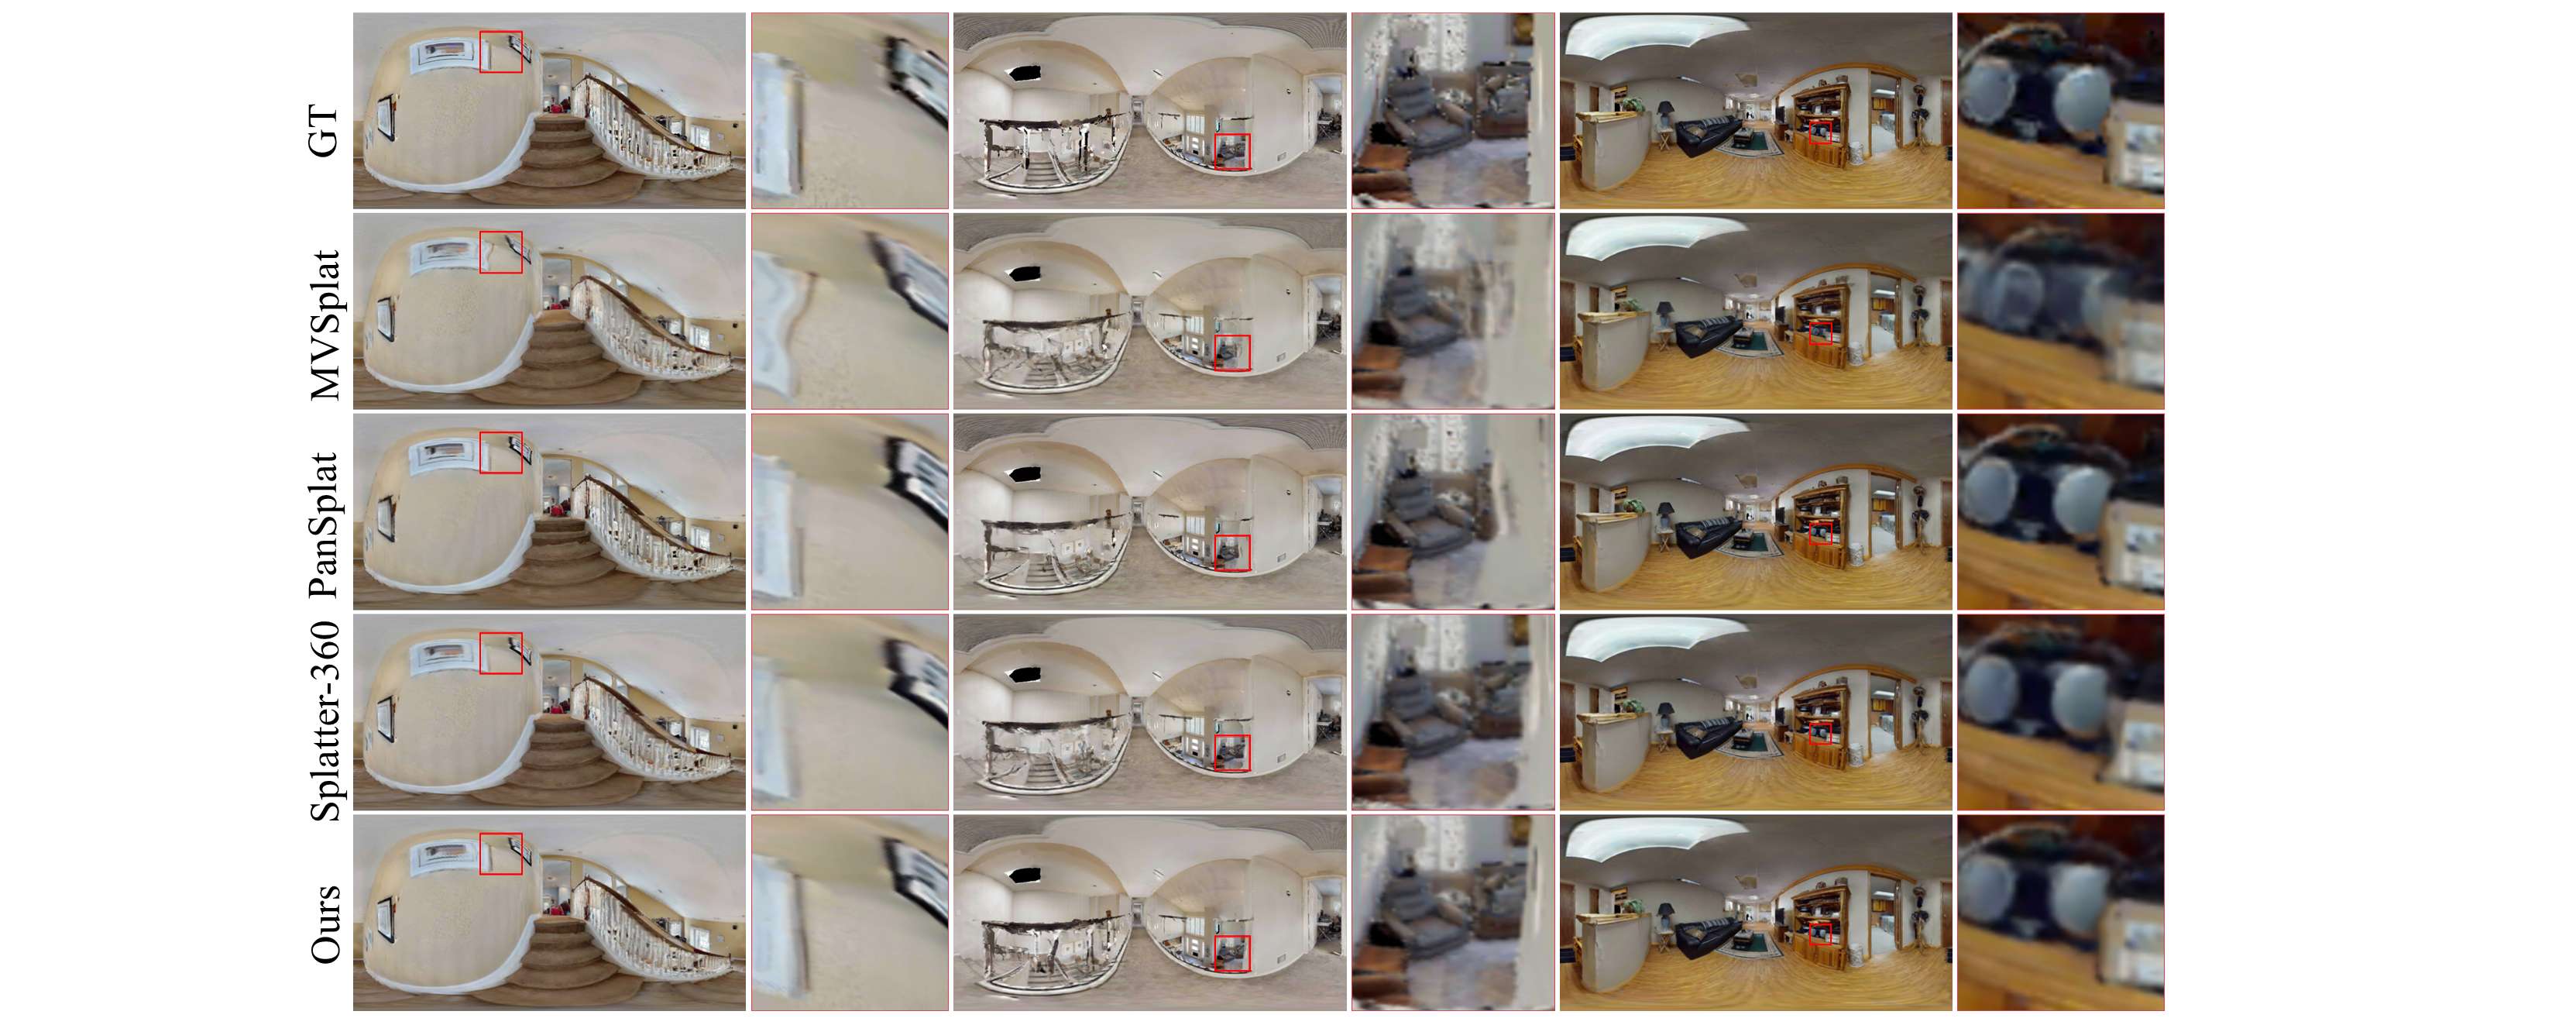
\includegraphics[width=\textwidth]{figures/small_rendering.png}
	\caption{Novel view rendering comparison of our method, Splatter-360, PanSplat, and MVSplat on the HM3D dataset.}
\label{fig:figure_placement}
\end{center}
\end{figure*}

\begin{figure*}[ht!]
\begin{center}
		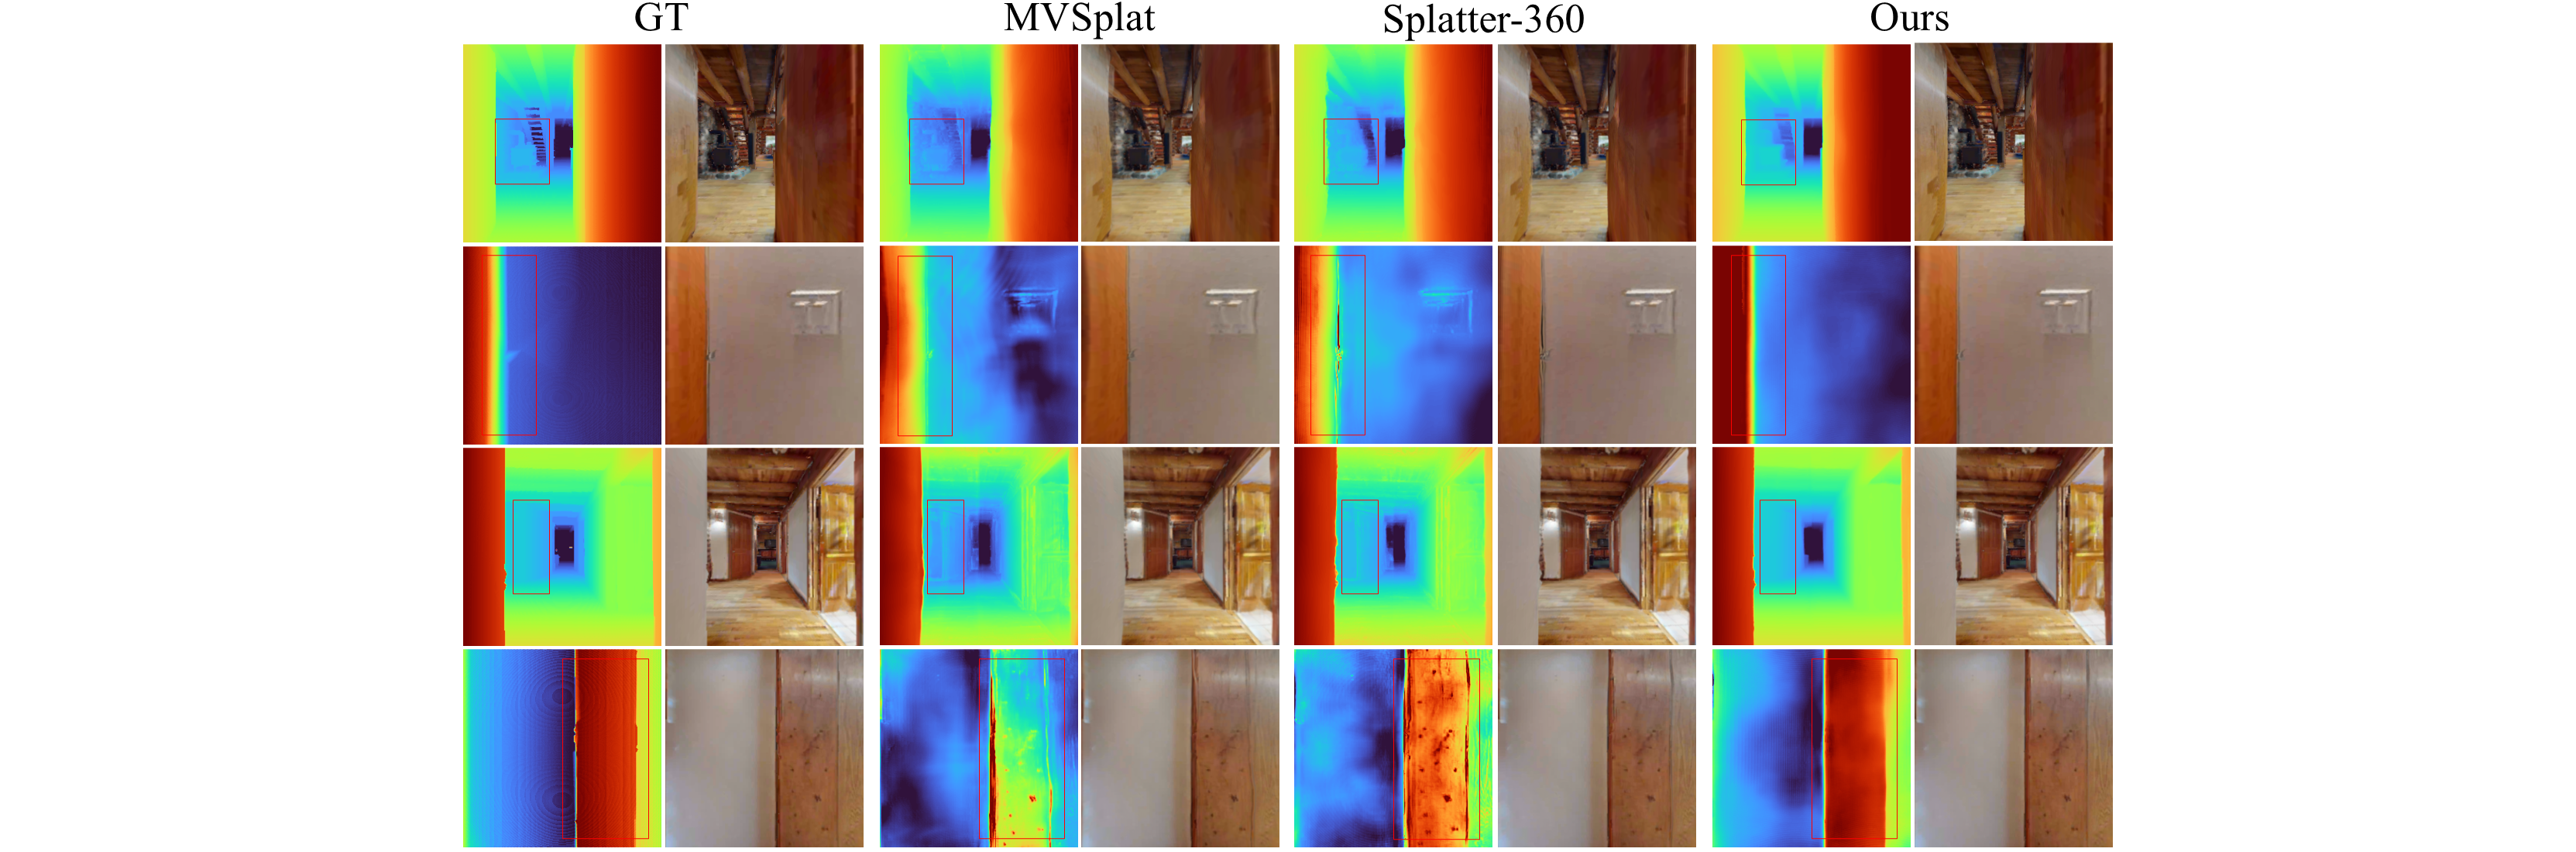
\includegraphics[width=\textwidth]{figures/small_depth.png}
	\caption{Novel view depth comparison among MVSplat, Splatter-360, and our method on the HM3D dataset.}
\label{fig:depth}
\end{center}
\end{figure*}

\subsection{Geometric Constraint}\label{subsec:D-Normal}
To enhance the geometric accuracy of feed-forward 3DGS predictions and better align Gaussian points with object surfaces, we introduce a geometric constraint.

\renewcommand{\arraystretch}{0.75} 
\begin{table*}[htbp]
  \centering  \captionsetup{justification=raggedright,singlelinecheck=false}
  \scriptsize    
  \caption{Quantitative comparison of depth estimation metrics on the HM3D and Replica datasets. $^\dagger$ indicates the model that was trained by us on the panoramic dataset. Best in each column is bolded.}
  \label{tab:depth}
  \begin{tabular}{lcccccccc}
    \toprule
    \multirow{2}{*}{Method}  & \multicolumn{4}{c}{HM3D} & \multicolumn{4}{c}{Replica} \\
    \cmidrule(lr){2-5} \cmidrule(lr){5-9}
           & Abs Diff$\downarrow$ & Abs Rel$\downarrow$ & RMSE$\downarrow$ & $\delta < 1.25$ $\uparrow$
           & Abs Diff$\downarrow$ & Abs Rel$\downarrow$ & RMSE$\downarrow$ & $\delta < 1.25$ $\uparrow$ \\
    \midrule
    MVSplat$^\dagger$ & 0.140 & 0.094 & 0.258 & 91.150 & 0.186 & 0.111 & 0.282 & 88.216 \\
    Splatter-360  & 0.098 & \textbf{0.068} & 0.193 & 95.417 & 0.103 & \textbf{0.068} & 0.185 & 95.412\\
    Ours & \textbf{0.053} & 0.069 & \textbf{0.141} & \textbf{96.423} & \textbf{0.055} & \textbf{0.068} & \textbf{0.138} & \textbf{96.528} \\
    \bottomrule
  \end{tabular}
\end{table*}

\subsubsection{Normal and Intersection Depth}\label{sec:Normal and Depth}
The spatial positions of feed-forward 3DGS points primarily depend on the estimated depth and are theoretically expected to lie on object surfaces. However, since Gaussians are represented as ellipsoids, their centers often deviate from the true surface, leading to geometric inconsistencies. To address this, we follow NeuSG and compress each ellipsoid along its smallest scale direction into a height-flattened form, allowing the Gaussian to better adhere to the underlying surface.

\renewcommand{\arraystretch}{0.75} 
\begin{table*}[htbp]
  \scriptsize
  \centering
    \caption{Quantitative comparison of novel view synthesis metrics on the HM3D and Replica datasets. Best in each column is bolded.}
  \label{tab:render}
  \setlength{\tabcolsep}{13pt}  
  \begin{tabular}{lcccccc}
    \toprule
    \multirow{2}{*}{Method}  & \multicolumn{3}{c}{HM3D} & \multicolumn{3}{c}{Replica} \\
    \cmidrule(lr){2-4} \cmidrule(lr){5-7}
           & PSNR$\uparrow$ & SSIM$\uparrow$ & LPIPS$\downarrow$
           & PSNR$\uparrow$ & SSIM$\uparrow$ & LPIPS$\downarrow$ \\
    \midrule
    MVSplat$^\dagger$ & 29.537 & 0.892 & 0.138  & 28.682 & 0.915 & 0.117 \\ 
    PanSplat     & 29.733 & \textbf{0.925} & 0.126 & \textbf{31.821} & \textbf{0.960} & 0.067 \\
    Splatter-360  & \textbf{31.669} & \textbf{0.925} & 0.100 & 31.584 & 0.952 & \textbf{0.064} \\
    Ours & 31.043 & 0.920 & \textbf{0.098} & 31.137 & 0.945 & 0.066 \\
    \bottomrule
  \end{tabular}
  \setlength{\tabcolsep}{6pt}
\end{table*}

Specifically, the scale factor $\mathbf{s}=(s_1,s_2,s_3)^T$ defines the ellipsoid’s extent along each principal axis. The normal vector $\mathbf{n}$ is then defined along the direction of the minimal scale component. Minimizing this component effectively flattens the ellipsoid, and a scale regularization loss $\mathcal{L}_\mathrm{s}$ is applied to constrain it towards zero:
\begin{equation}\label{equ:6}
\mathcal{L}_\mathrm{s}=\|\min(s_1,s_2,s_3)\|_1.\end{equation}

In depth computation, conventional methods typically obtain the depth from the center position $\textbf{p}=(p_x,p_y,p_z)$ of each Gaussian in the camera coordinate system. However, this ignores the normal vector $\textbf{n}$ and thus limits the effectiveness of geometric constraints. We therefore adopt a more appropriate approach, computing the intersection depth between the camera ray $\textbf{r}$ and the flattened Gaussian surface, defined as:
\begin{equation}\label{equ:7}
\mathbf{d}(\mathbf{n},\mathbf{p})={r_z(\mathbf{n}\cdot \mathbf{p})}/{(\mathbf{n}\cdot \mathbf{r})},
\end{equation}
Here, $r_z$ denotes the z-component of the ray $\textbf{r}$. The intersection depth depends on both the position $\textbf{p}$ and the normal vector $\textbf{n}$ of the Gaussian, allowing them to be jointly constrained during optimization to improve depth estimation accuracy.

\subsubsection{D-Normal Regularization}\label{sec:D-Normal formula}
Following this approach, we adopt the D-Normal regularization. Specifically, a depth map is generated using the 3DGS renderer, following a procedure analogous to RGB rendering.
\begin{equation}
\label{equ:8}
\hat{D}={\sum_{i\in M} d_i\,\alpha_i\, T_i}/({\sum_{i\in M} \alpha_i\, T_i})
\qquad\quad
T_i=\prod_{j=1}^{i-1}(1-\alpha_j)
\end{equation}
where $d_i$ is the intersection depth from \eqref{equ:7} and $M$ is the number of Gaussians the ray passes through. Subsequently, the rendered normal 
$\bar{\textbf{N}}_{d}(\textbf{n},\textbf{p})$ is obtained by computing finite differences of the depth map along the horizontal and vertical directions and taking their cross product. This normal depends on both the Gaussian normal $\textbf{n}$ and the position 
$\textbf{p}$:
\begin{equation}\label{equ:9}
\bar{\mathbf{N}}_{d}(\mathbf{n},\mathbf{p})=\frac{\nabla_{v}\mathbf{d}(\mathbf{n},\mathbf{p})\times\nabla_{h}\mathbf{d}(\mathbf{n},\mathbf{p})}{|\nabla_{v}\mathbf{d}(\mathbf{n},\mathbf{p})\times\nabla_{h}\mathbf{d}(\mathbf{n},\mathbf{p})|}.
\end{equation}
The D-Normal regularization enforces consistency between the rendered normal $\bar{\mathbf{N}}_{d}$ and the target normal $\mathbf{N}$, enabling joint optimization of Gaussian positions and orientations, as illustrated in Fig.~\ref{fig:surface}. The regularization loss is formulated as:
\begin{equation}\label{equ:10}
\mathcal{L}_{\mathrm{dn}}=\|\bar{\mathbf{N}}_{d}-\mathbf{N}\|_{1}+(1-\bar{\mathbf{N}}_{d}\cdot\mathbf{N}).
\end{equation}
Our overall loss function is defined as:
\begin{equation}
\mathcal{L}_{\mathrm{total}}=\mathcal{L}_{\mathrm{rgb}}+\lambda_{1}\mathcal{L}_{\mathrm{s}}+\lambda_{2}\mathcal{L}_{\mathrm{depth}}+\lambda_{3}\mathcal{L}_{\mathrm{dn}}.
\end{equation}

\begin{figure}[tbp]
  \centering  \captionsetup{width=\columnwidth,justification=justified,singlelinecheck=false}
  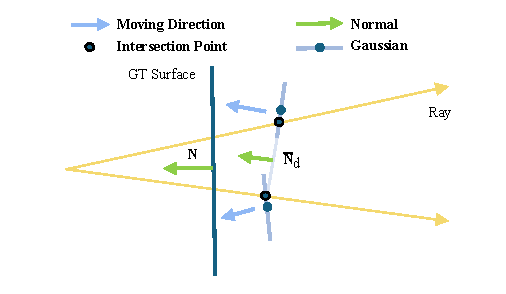
\includegraphics[width=8cm]{figures/surface.eps}
  \caption{Illustration of the D-Normal regularization. $\bar{\mathbf{N}}_{d}$ is supervised by the ground-truth normal through $\mathcal{L}_{\mathrm{dn}}$(defined in subsection~\ref{sec:D-Normal formula} ), guiding the flattened Gaussians to better fit the true surface.}
  \label{fig:surface}
\end{figure}
